\section{TINJAUAN PUSTAKA}

% Ubah konten-konten berikut sesuai dengan isi dari tinjauan pustaka
\subsection{Hasil penelitian terdahulu}
\subsubsection{Rancang Bangun Anemometer Ultrasonik dalam Ruangan}
Penelitian yang dilakukan oleh Ahmad Harris Abdillah dengan judul 'Rancang Bangun Anemometer Ultrasonik dalam Ruangan' \parencite{Newton1687} 
membuat rancang bangun anemometer ultrasonic dalam ruangan. Dari alat tersebut sudah bisa memberikan data yang cukup baik, namun masih dapat 
ditingkatkan akurasinya dan ukuran dari alatnya masih terlalu besar untuk diaplikasikan didalam ruangan.

\begin{figure}[h!]
	\label{abdillah_anemo_skema}
	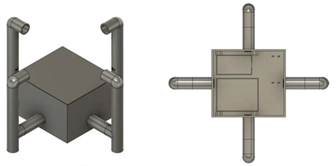
\includegraphics[width=\linewidth]{gambar/fig_anemometer_abdillah_skema}
	\caption{Alat Anemometer Ultrasonic di dalam ruangan \parencite{Abdillah2022}}
\end{figure}

\subsubsection{Rancang Bangun \emph{Thermal-Based Anemometer} dan Arah Angin untuk Aliran Udara Rendah}

\subsubsection{Sistem Pendeteksi Arah Angin Menggunakan \textit{Hot-Wire} Anemometer}

\subsubsection{Simulator Sensor Pengukur Jarak Berbasis Ultrasonic dan Infrared Menggunakan Kendali Jarak Jauh Dilengkapi Webcam Berbasis Web 
Interface}


\subsection{Angin}

% Contoh penggunaan referensi dari pustaka
Angin adalah udara yang bergerak dari daerah yang bertekanan udara tinggi (maksimum) ke daerah yang bertekanan udara rendah (minimum). Perbedaan 
tekanan udara di sebebabkan adanya perbedaan suhu udara. Apabila suhu udaranya tinggi maka tekanan udaranya minimum, sedangkan apabila suhu udaranya 
rendah maka tekanan udara maksimum. Alat utuk mengukur arah dan kecepatan angin adalah anemometer.

Faktor terjadinya Angin dalam proses terjadinya angin dipengaruhi oleh beberapa faktor yang menyebabkan angin muncul antara lain sebagai berikut. 
Gradien Barometris, adalah bilang yang menampilkan adanya perbedaan tekanan udara dari 2 isobar pada jarak 111 km. Dimana semakin besar gradien 
barometris, maka semakin cepat juga tiupan angin. Letak Tempat, adalah angin lebih cepat yang berada atau dekat di garis khatulistiwa, dari pada yang 
jauh dari khatulistiwa. Tinggi Tempat,Tinggi rendahnya tempat/lokasi dapat mempengaruhi karena semakin tinggi tempat tersebut, maka semakin kencang 
angin bertiup, dan sebaliknya, Hal ini dapat terjadi karena disebabkan oleh pengaruh gaya gesekan yang menghambat laju udara.

Di permukaan yang tidak merata seperti gunung, pohon dan tempat lainnya memberikan gaya gesekan yang besar. Waktu, Disiang hari angin bergerak lebih 
cepat dari pada di malam hari. Dalam klimatologi, angin memiliki dua fungsi dasar yaitu : Pemindahan panas baik dalam bentuk yang dapat diukur maupun 
yang tersimpan dari lintang rendah ke lintang yang lebih tinggi dan akan membuat setimbang neraca radiasi surya antara lintang rendah dan tinggi 
Pemindahan uap air yang dievaporasikan dari laut ke daratan dimana sebagian besar dikondensasikan untuk menyediakan kebutuhan air yang turun kembali 
sebagai hujan, kabut ataupun embun.fungsi angin secara umum juga adalah memindahkan uap air yang sudah terevaporasi dari laut ke daratan dan mengalamu 
kondensasi yang selanjutnya menjadi hujan.

\subsection{Anemometer}

Anemometer adalah alat untuk mengukur atau menentukan kecepatan angin. Anemometer merupakan salah satu instrument yang sering 
digunakan oleh Badan Meterologi Klimatologi dan Geofisika (BMKG). Kata anemometer berasal dari Bahasa Yunani anemos yang berarti angin, angin 
merupakan udara yang bergerak ke segala arah, angin bergerak dari suatu tempat menuju ke tempat yang lain. Anemometer ini pertama kali diperkenalkan 
oleh Leon Batista Alberti dari italia pada tahun 1450. Pada saat itu, model yang digunakan adalah Cup Anemometer.

\subsubsection{Cup Anemometer}
	Cup Anemometer adalah alat yang mempunyai baling-baling berbentuk setengah lingkaran dan menyerupai mangkok kecil. Ketika tertiup angin, mangkok 
  yang terdapat pada anemometer akan bergerak sesuai arah angin. Makin besar kecepatan angin meniup mangkok tersebut, makin cepat pula kecepatan 
  berputarnya piringan mangkok tersebut, makin cepat pula kecepatan berputarnya piringan mangkok. Dari jumlah putaran dalam satu detik maka dapat 
  diketahui kecepatananginnya. Didalam anemometer terdapat alat pencacah yang akan menghitung kecepatan angin.
	
	\subsubsection{Windmill Anemometer}
	
	Windmill Anemometer adalah anemometer di mana kincir angin didorong oleh aliran udara, dan rotasi ditransmisikan melalui gearing ke dial atau 
  mekanisme perekaman lainnya. Dalam beberapa instrumen, baling-baling dan dial yang berputar berada pada bidang yang sama yaitu, keduanya vertikal, 
  sementara di lain dial adalah horizontal. Dalam jenis kincir angin, pengoperasian pengukuran udara melibatkan pembacaan dial pada awal dan akhir 
  periode yang diukur. Instrumen kincir angin dapat dilengkapi dengan pegangan ekstensi, menyediakan bentuk kendali jarak jauh; digunakan untuk mengukur 
  kecepatan udara di tempat yang tidak dapat diakses.
	
	\subsubsection{Hot Wire/Thermal Anemometer}
	
	Thermal Anemometer atau dikenal juga dengan Hot Wire Anemometer adalah transduser termal yang banyak digunakan untuk mengukur kecepatan aliran udara 
  sesaat. Penggunaan anemometer hot wire memungkinkan kecepatan aliran sesaat dihitung dari pengukuran tegangan listrik [Kim et al., 2016]. Keuntungan 
  dari anemometer hot wire dikaitkan dengan resolusi spasial yang sangat tinggi dan karakteristik respons frekuensi yang sangat baik.
	
	\subsubsection{Ultrasonic Anemometer}
	
	Time of flight pulsa suara yang merambat di udara menyediakan metode lebih lanjut untuk merasakan kecepatan angin. Ultrasound dapat dengan mudah 
  dihasilkan dan dideteksi secara elektronik, dan digunakan untuk pengukuran tersebut. Dalam anemometer ultrasonik, waktu terbang yang diperlukan 
  pulsa ultrasound untuk bergerak maju dan mundur antara dua transduser tetap A dan B diukur. Karena responnya yang cepat, anemometer sonik sangat 
  cocok untuk pengukuran lapangan fluktuasi turbulen kecepatan angin, dan dalam beberapa arah secara bersamaan. vektor kecepatan tiga dimensi dapat 
  dihitung dengan beberapa pengolahan data dan identitas trigonometri (Harrison, 2014).
	
	Satu-satunya kelemahan signifikan dari instrumen ini adalah biaya dan pengelolaan volume data yang besar yang dapat dihasilkan dengan cepat. 
  Anemometer ultrasonik berfungsi untuk mengukur kecepatan dan arah angin. Didesain tanpa ada bagian yang bergerak, anemometer ultrasonik ini 
  diharapkan lebih handal, bebas perawatan, tahan lama, dan dapat beroperasi dalam kondisi cuaca yang ekstrim. Untuk tugas akhir ini dibatasi 
  sampai dengan pembuatan prototipe awal dan pembuktian bahwa sinyal ultrasonik akan berubah time of flight (ToF) nya ketika tranduser ultrasonik 
  dihembus oleh angin.

\subsection{Gelombang Ultrasonic}
Suara/akustik merupakan energi mekanik yang menyebar melalui suatu medium yang kontinu dan elastis dengan memampatkan dan menipiskan partikel 
sehingga mengubah susunannya. Ada dua tipe dasar dari gelombang akustik, yaitu gelombang longitudinal dan gelombang transversal. Pada gelombang 
longitudinal, gerak partikel pada suatu media akustik searah dengan perambatannya. Pada gelombang transversal,pergerakan partikelnya tegak lurus dengan arah rambatnya.

\begin{figure}[h!]
	\centering
	\includegraphics[width=0.7\linewidth]{"gambar/spektrum akustik"}
	\caption{Spektrum Akustik}
	\label{fig:spektrum-akustik}
\end{figure}

Gelombang ultrasonik merupakan gelombang mekanik longitudinal yang frekuensinya melampaui batas dengar telinga manusia (di atas 20 kHz), dan 
gelombangnya menyebar dalam medium baik padat, cair dan gas, yang disebabkan oleh osilasi bolak balik partikel pada titik kesetimbangan. 
Pada spektrum akustik seperti yang diperlihatkan oleh Gambar \ref{fig:spektrum-akustik}, gelombang ultrasonik berada pada sisi kanan spektrum akustik.

Pada frekuensi 10 kHz - 150 kHz, ultrasonik dipakai untuk komunikasi beberapa binatang seperti kelelawar dan lumba-lumba. Jika pada frekuensi ini 
dayanya ditingkatkan maka ultrasonic dapat dipakai untuk membantu proses pembersihan (cleaner) beberapa material misalkan perhiasan.Untuk aplikasi 
medical imaging dibutuhkan frekuensi dari 1 MHz sampai dengan 20 MHz misalkan seperti yang dipakai untuk ultrasonografi (USG).

\subsection{Perambatan Gelombang Ultrasonic}

Gelombang ultrasonik yang dihasilkan oleh transduser dapat berupa sinyal pulsa atau sinyal kontinu, tergantung pada tegangan yang diinputkan pada 
transduser. Mode apa yang akan dipakai tergantung pada metode tes yang akan digunakan. 

Karakteristik gelombang ultrasonik yang melalui medium mengakibatkan getaran partikel dengan medium amplitudo sejajar dengan arah rambat secara 
longitudinal sehingga menyebabkan partikel medium membentuk rapatan (strain) dan tegangan (stress). Proses kontinu yang menyebabkan terjadinya rapatan 
dan regangan di dalam medium disebabkan oleh getaran partikel secara periodic selama gelombang ultrasonik melaluinya (Resnick et al., 1992).

Gelombang ultrasonik di dalam material dapat merambat dengan tiga macam pola gelombang yang sering digunakan, yaitu gelombang longitudinal, 
gelombang transversal, gelombang permukaan atau Rayleigh waves. 

Gelombang longitudinal merupakan gelombang yang paling sering digunakan untuk pengujian ultrasonik. Kelebihan gelombang ini adalah kemampuannya 
yang dapat merambat di dalam zat cair dan gas, sama baiknya seperti pada material solid. Mekanisme gelombang ini adalah perambatannya sejajar 
dengan arah gerakan atom yang digetarkan.

\begin{figure}
	\centering
	\includegraphics[width=0.7\linewidth]{"gambar/pergerakan partikel"}
	\caption{Pergerakan partikel akibat gelombang longitudinal (kiri) dan gelombang transversal (kanan) (k arah pergerakan gelombang, l jarak 
  antara atom yang bersebelahan) (Still, 2009)}
	\label{fig:pergerakan-partikel}
\end{figure}

Gelombang transversal merupakan jenis gelombang yang juga sering digunakan, tetapi tidak seperti gelombang longitudinal, gelombang ini sulit 
merambat dalam zat cair dan gas, karena karakternya yang kurang elastis dan dibutuhkan gaya yang kuat pada partikel untuk berosilasi. Gelombang 
ini dapat terjadi apabila gelombang ultrasonik merambat pada arah yang tegak lurus, dengan vibrasi yang bergerak ke atas dan ke bawah, pada arah 
dan bidang gerakan atom yang digetarkan. Ilustrasi dari gelombang ini secara skematis ditunjukkan pada Gambar \ref{fig:pergerakan-partikel} yang 
menunjukkan pergerakan partikel berpengaruh terhada perambatan dari gelombang longitudinal dan transversal.

\subsection{Sensor Jarak Ultrasonik}

Sensor ultrasonik adalah sebuah sensor yang mengubah besaran fisis (bunyi) menjadi besaran listrik. Sensor ultrasonik ini menggunakan ultrasound, 
dimana ia menggunakan frekuensi suara yang sangat tinggi diatas batas pendengaran manusia. Rata-rata manusia mempunyai batas pendengaran sekitar 20 
KHz, sehingga sensor menggunakan batas diatas pendengaran manusia. Pulsa dari gelombang suara ultrasonik dikirim dari transducer dan kemudian diambil 
lagi menggunakan transducer yang sama ketika memantul ke sebuah objek. Dari kalkulasi waktu yang digunakan untuk suatu pulsa dapat kembali ditunjukkan 
pada Gambar 2.x. Kecepatan pengiriman gelombang suara di udara kering pada suhu 20 Celsius adalah 340 m/s.

\begin{figure}[h!]
	\centering
	\includegraphics[width=0.7\linewidth]{"gambar/diagram kerja sensor ultrasonic"}
	\caption{Prinsip jarak sonar atau radar pengukuran.}
	\label{fig:diagram-kerja-sensor-ultrasonic}
\end{figure}

Pada sensor ini gelombang ultrasonik dibangkitkan melalui sebuah benda yang disebut piezoelektrik. Piezoelektrik ini akan menghasilkan gelombang 
ultrasonik dengan frekuensi 40 kHz. Sensor ultrasonik secara umum digunakan untuk suatu pengungkapan tak sentuh yang beragam seperti aplikasi 
pengukuran jarak. Bentuk fisik dari sensor ultrasonik seperti pada Gambar \ref{fig:sensor-ultrasonic}

\begin{figure}[h!]
	\centering
	\includegraphics[width=0.7\linewidth]{"gambar/sensor ultrasonic"}
	\caption{Modul HC-SR04.}
	\label{fig:sensor-ultrasonic}
\end{figure}

Modul HC-SR04 memiliki 4 kaki pin yaitu pin Vcc, pin Trig, pin Echo, dan pin GND dengan fungsi yang berbeda-beda. Pada pin Vcc berfungsi 
sebagai pemberi tegangan ke sensor ultrasonik. Pin Trig atau sama dengan pin trigger adalah pin yang berfungsi sebagai pemicu untuk memantulkan 
sinyal pantul. Sedangkan pada pin echo berfungsi sebagai pin receiver atau pin penerima dari sinyal pantul yang dihasilkan oleh pin trigger. 
Dan pin GND atau sama dengan pin ground berfungsi sebagai pin penetral.

\begin{table}
	\caption{Spesifikasi HC-SR04}
	\centering
	\begin{tabular}{|c|c|}
		\hline
		Working Voltage & DC 5V \\
		\hline
		Working Current & 15mA \\
		\hline
		Working Frequency & 40 KHz \\
		\hline
		Max Range & 4m \\
		\hline
		Min Range & 2cm \\
		\hline
		Measuring Angle & 15 \\
		\hline
		Trigger Input Signal &  TTL Pulse \\
		\hline
		Echo Output Signal & Input TTL lever signal and the range in proportion \\
		\hline
		Dimension & 45*20*15 mm \\
		\hline
	\end{tabular}
\end{table}

Karena sistem kerja sensor jarak ultrasonik ini adalah dengan menggunakan cara menembakkan gelombang ke objek dan menunggu 
pantulannya maka membutuhkan waktu tempuhnya dua kali, sehingga untuk mengetahui jarak sebenarnya harus dibagi dua. Dimana 
jarak setengah awal adalah waktu gelombang ditembakkan dan mengenai obyek, jarak setengah berikutnya adalah pantulan 
gelombang dari obyek yang kembali ke receiver. Jarak yang diukur menggunakan rumus seperti pada Persamaan 2.1.

\begin{equation}\label{rumus jarak}
	 S= V * t : 2
\end{equation}

Dimana S adalah jarak antara pemancar dan penerima dalam satuan meter (m), V adalah kecepatan suara yaitu 340 m/s, t adalah 
waktu tempuh dalam satuan detik (s).

\subsection{Time of Flight (ToF)}

Time of Flight adalah pengukuran waktu yang diperlukan oleh suatu benda, partikel atau gelombang (baik akustik, elektromagnetik, 
dll.) untuk menempuh jarak melalui media. Informasi ini kemudian dapat digunakan untuk mengukur kecepatan atau panjang lintasan, 
atau sebagai cara untuk mempelajari tentang sifat partikel atau medium (seperti komposisi atau laju aliran). 

Miguel Perez del Valle, Jose Antonio Urbano Castelan, Yasuhiro Matsumoto, dan Rau’l Cortes Mateos dalam penelitiannya menyatakan 
Kecepatan rambat suara di udara dipengaruhi oleh komponen kecepatan aliran udara(angin). Jika angin mengalir dalam arah rambat 
suara maka akan meningkatkan kecepatan rambat suara, sedangkan jika angin mengalir berlawanan dengan arah rambat suara, maka 
kecepatan rambat suara akan menurun (del Valle et al., 2007).

\subsection{Raspberry Pi Pico W}

